\documentclass[border=10pt]{standalone}
\usepackage{amsmath,amssymb}
\usepackage{tikz}
\usetikzlibrary{arrows.meta,decorations.pathreplacing,calc,positioning,
  patterns,fit}

\begin{document}
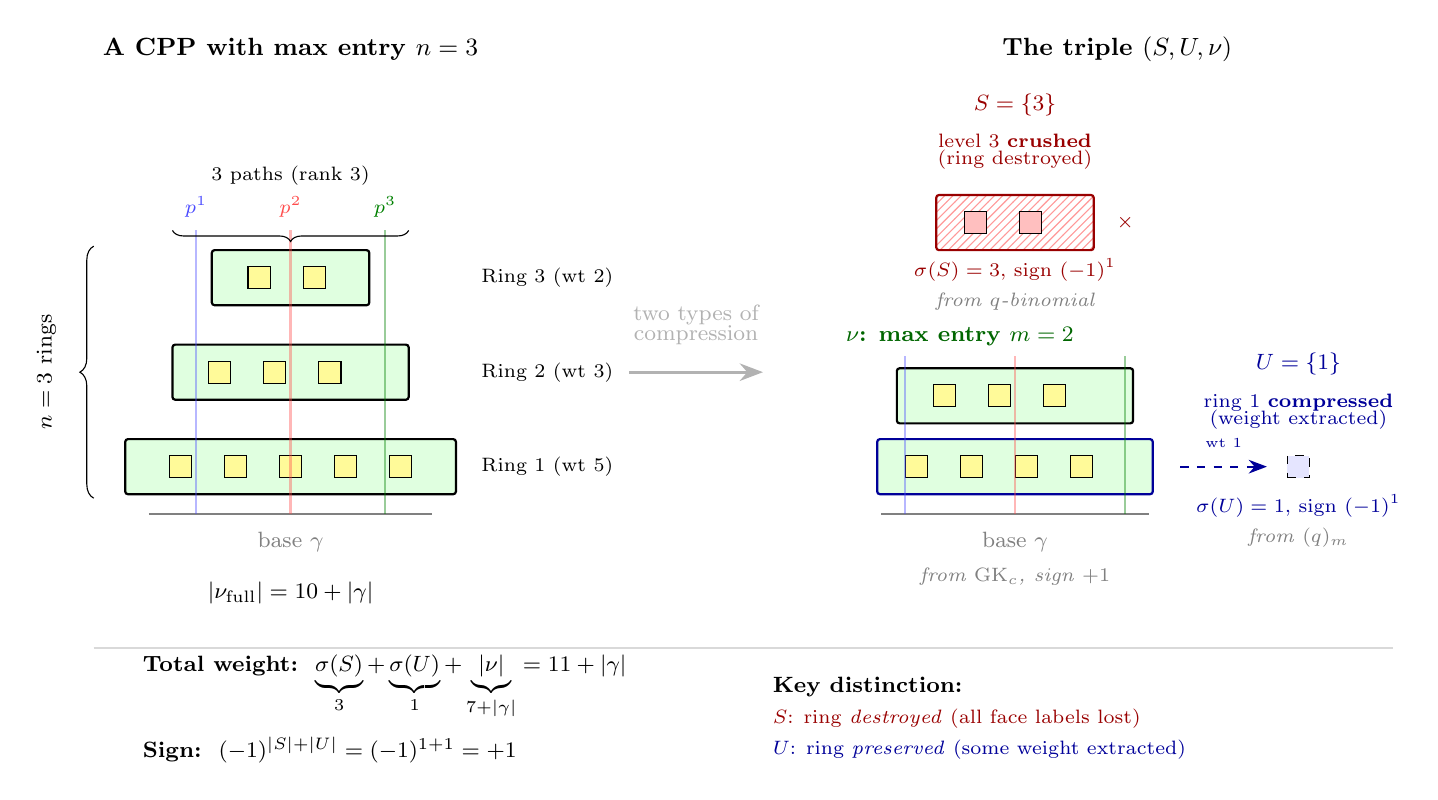
\begin{tikzpicture}[
  >=Stealth,
  lbl/.style={font=\footnotesize},
  slbl/.style={font=\scriptsize},
  title/.style={font=\bfseries\small},
  % Ring styles
  ring/.style={draw, thick, minimum height=0.7cm, rounded corners=1pt},
  ringfill/.style={ring, fill=green!12},
  ringcrush/.style={ring, pattern=north east lines, pattern color=red!40,
    draw=red!60!black},
  ringextract/.style={ring, fill=green!12, draw=blue!60!black},
  % Cube styles
  cube/.style={draw, fill=yellow!40, minimum size=0.28cm, inner sep=0,
    font=\tiny},
  cubeghost/.style={draw, dashed, fill=blue!10, minimum size=0.28cm,
    inner sep=0},
  cubered/.style={draw, fill=red!25, minimum size=0.28cm, inner sep=0},
]

%% ============================================================
%% PANEL A: The full CPP (left)
%% ============================================================
\node[title] at (2, 5.8) {A CPP with max entry $n = 3$};

% Ring 1 (bottom): 5 cubes
\node[ringfill, minimum width=4.2cm] (A1) at (2, 0.5) {};
\foreach \i in {0,...,4} {
  \node[cube] at (0.6 + 0.7*\i, 0.5) {};
}
\node[slbl, right] at (4.3, 0.5) {Ring 1 (wt 5)};

% Ring 2: 3 cubes
\node[ringfill, minimum width=3cm] (A2) at (2, 1.7) {};
\foreach \i in {0,...,2} {
  \node[cube] at (1.1 + 0.7*\i, 1.7) {};
}
\node[slbl, right] at (4.3, 1.7) {Ring 2 (wt 3)};

% Ring 3: 2 cubes
\node[ringfill, minimum width=2cm] (A3) at (2, 2.9) {};
\foreach \i in {0,1} {
  \node[cube] at (1.6 + 0.7*\i, 2.9) {};
}
\node[slbl, right] at (4.3, 2.9) {Ring 3 (wt 2)};

% Base
\draw[thick, gray] (0.2, -0.1) -- (3.8, -0.1);
\node[lbl, gray] at (2, -0.45) {base $\gamma$};

% The 3 lattice paths
\draw[thick, blue!70, opacity=0.4] (0.8, -0.1) -- (0.8, 3.5);
\draw[thick, red!70, opacity=0.4] (2.0, -0.1) -- (2.0, 3.5);
\draw[thick, green!50!black, opacity=0.4] (3.2, -0.1) -- (3.2, 3.5);
\node[slbl, blue!70] at (0.8, 3.8) {$p^1$};
\node[slbl, red!70] at (2.0, 3.8) {$p^2$};
\node[slbl, green!50!black] at (3.2, 3.8) {$p^3$};

% Label: 3 paths
\draw[decorate, decoration={brace, amplitude=4pt, mirror}]
  (0.5, 3.5) -- (3.5, 3.5);
\node[slbl] at (2, 4.2) {3 paths (rank 3)};

% Label: 3 rings
\draw[decorate, decoration={brace, amplitude=5pt}]
  (-0.5, 0.1) -- (-0.5, 3.3);
\node[lbl, rotate=90] at (-1.1, 1.7) {$n = 3$ rings};

% Total weight
\node[lbl] at (2, -1.1) {$|\nu_{\text{full}}| = 10 + |\gamma|$};


%% ============================================================
%% Arrow
%% ============================================================
\draw[->, very thick, gray!60] (6.3, 1.7) -- (8.0, 1.7);
\node[lbl, gray!60, align=center] at (7.15, 2.3) {two types of\\[-2pt]
  compression};


%% ============================================================
%% PANEL B: The triple (S, U, nu) — right side
%% ============================================================
\node[title] at (12.5, 5.8) {The triple $(S, U, \nu)$};

% --- S component (top right) ---
\node[lbl, red!60!black, font=\footnotesize\bfseries] at (11.2, 5.1)
  {$S = \{3\}$};
\node[slbl, red!60!black, align=center] at (11.2, 4.5)
  {level 3 \textbf{crushed}\\[-2pt](ring destroyed)};

% Show the crushed ring
\node[ringcrush, minimum width=2cm] at (11.2, 3.6) {};
\foreach \i in {0,1} {
  \node[cubered] at (10.7 + 0.7*\i, 3.6) {};
}
\node[slbl, red!60!black] at (12.6, 3.6) {$\times$};

% Contribution
\node[slbl, red!60!black] at (11.2, 3.0)
  {$\sigma(S) = 3$, sign $(-1)^1$};

% From label
\node[slbl, gray] at (11.2, 2.6)
  {\itshape from $q$-binomial};


% --- U component (right of tower) ---
\node[lbl, blue!60!black, font=\footnotesize\bfseries] at (14.8, 1.8)
  {$U = \{1\}$};
\node[slbl, blue!60!black, align=center] at (14.8, 1.2)
  {ring 1 \textbf{compressed}\\[-2pt](weight extracted)};

% Show the extracted cube
\node[cubeghost] at (14.8, 0.5) {};
\draw[->, blue!60!black, thick, dashed] (13.3, 0.5) -- (14.4, 0.5);
\node[slbl, blue!60!black] at (13.85, 0.8) {\tiny wt 1};

% Contribution
\node[slbl, blue!60!black] at (14.8, 0.0)
  {$\sigma(U) = 1$, sign $(-1)^1$};

% From label
\node[slbl, gray] at (14.8, -0.4)
  {\itshape from $(q)_m$};


% --- nu component (the remaining tower) ---
\node[lbl, green!40!black, font=\footnotesize\bfseries] at (10.5, 2.15)
  {$\nu$: max entry $m = 2$};

% Ring 1 of nu: 4 cubes (one extracted to U)
\node[ringextract, minimum width=3.5cm] (B1) at (11.2, 0.5) {};
\foreach \i in {0,...,3} {
  \node[cube] at (9.95 + 0.7*\i, 0.5) {};
}
\node[slbl, right] at (13.1, 0.5) {};

% Ring 2 of nu: 3 cubes (was ring 2 of original; ring 3 was crushed)
\node[ringfill, minimum width=3cm] (B2) at (11.2, 1.4) {};
\foreach \i in {0,...,2} {
  \node[cube] at (10.3 + 0.7*\i, 1.4) {};
}

% Base
\draw[thick, gray] (9.5, -0.1) -- (12.9, -0.1);
\node[lbl, gray] at (11.2, -0.45) {base $\gamma$};

% Paths (only 2 now since m=2)
\draw[thick, blue!70, opacity=0.4] (9.8, -0.1) -- (9.8, 1.9);
\draw[thick, red!70, opacity=0.4] (11.2, -0.1) -- (11.2, 1.9);
\draw[thick, green!50!black, opacity=0.4] (12.6, -0.1) -- (12.6, 1.9);

% From label
\node[slbl, gray] at (11.2, -0.9) {\itshape from $\mathrm{GK}_c$,
  sign $+1$};


%% ============================================================
%% Weight / sign summary (bottom)
%% ============================================================
\draw[thick, gray!30] (-0.5, -1.8) -- (16, -1.8);

\node[lbl, anchor=west] at (0, -2.3) {%
  \textbf{Total weight:}\;
  $\underbrace{\sigma(S)}_{3}
   + \underbrace{\sigma(U)}_{1}
   + \underbrace{|\nu|}_{7 + |\gamma|}
   = 11 + |\gamma|$};

\node[lbl, anchor=west] at (0, -3.1) {%
  \textbf{Sign:}\; $(-1)^{|S|+|U|} = (-1)^{1+1} = +1$};

\node[lbl, anchor=west] at (8, -2.3) {%
  \textbf{Key distinction:}};
\node[slbl, anchor=west, red!60!black] at (8, -2.7) {%
  $S$: ring \emph{destroyed} (all face labels lost)};
\node[slbl, anchor=west, blue!60!black] at (8, -3.1) {%
  $U$: ring \emph{preserved} (some weight extracted)};

\end{tikzpicture}
\end{document}
